% Especificaciones del tamaño de letra, tamaño de hoja, márgenes, librerias, etc.
\documentclass[12pt, letterpaper]{article}
\usepackage[english]{babel}
\usepackage[utf8]{inputenc}
\usepackage[T1]{fontenc}
\usepackage{amsmath}
\usepackage{graphicx}
\usepackage{subcaption}
\usepackage{hyperref}
\usepackage{url}
\usepackage{amssymb}
\usepackage{float}
\usepackage[margin=1in]{geometry}
\renewcommand{\baselinestretch}{1.5}

% Enlace Bibliografía
\usepackage{csquotes}
\usepackage[notes,backend=biber]{biblatex-chicago}
\addbibresource{referencias.bib}

% Titulo, autores, fecha.
\title{Práctica \#4: Análisis y Control de un Sistema Dinámico}
\author{Carlos Vásquez 1155057}

% Inicio del documento
\begin{document}
\maketitle
\section*{Introducción}
En la práctica anterior se realizó el modelo matemático de un péndulo simple a través de una ecuación diferencial y posteriormente se llevó a cabo el diagrama de bloque en SIMULINK para su manipulación rápida y efectiva.

\begin{figure}[H]
	\centering
	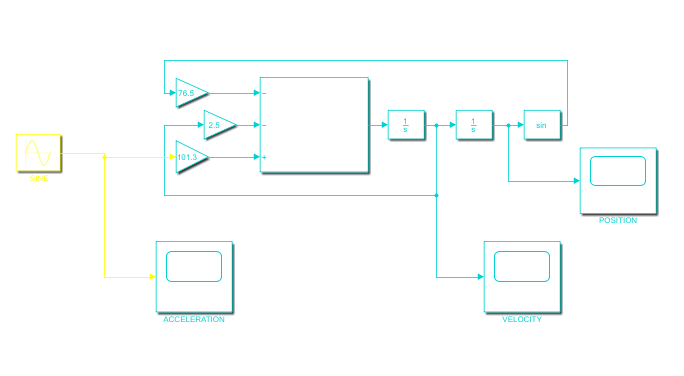
\includegraphics[width=0.7\textwidth]{pendulum.png}
	\caption{Representación de un péndulo con diagramas de bloque.}
\end{figure}

A pesar de la correcta representación del sistema dinámico, es complicado conseguir la estabilidad del sistema por sí mismo, en especial si se consideran señales que perturben al sistema como tal. Es por eso que la realización de controladores es tan importante en el diseño de sistemas capaces de encontrar y corregir errores.

El simple hecho de tener amortiguamiento (ya sea por aire o algún otro fluido de viscosidad conocida) afectará a nuestro sistema y su desempeño. Dado que todos los sistemas físicos cuentan con limitaciones e interacciones con su entorno, es imposible aislarlos para obtener lo que se idealiza a través del modelado matemático. El controlador se encargará de registrar estos cambios y realizar una comparación para así poder cambiar la señal en cuestión y modificarla con la finalidad de obtener un sistema que sea estable a lo largo del tiempo.

\begin{figure}[H]
	\centering
	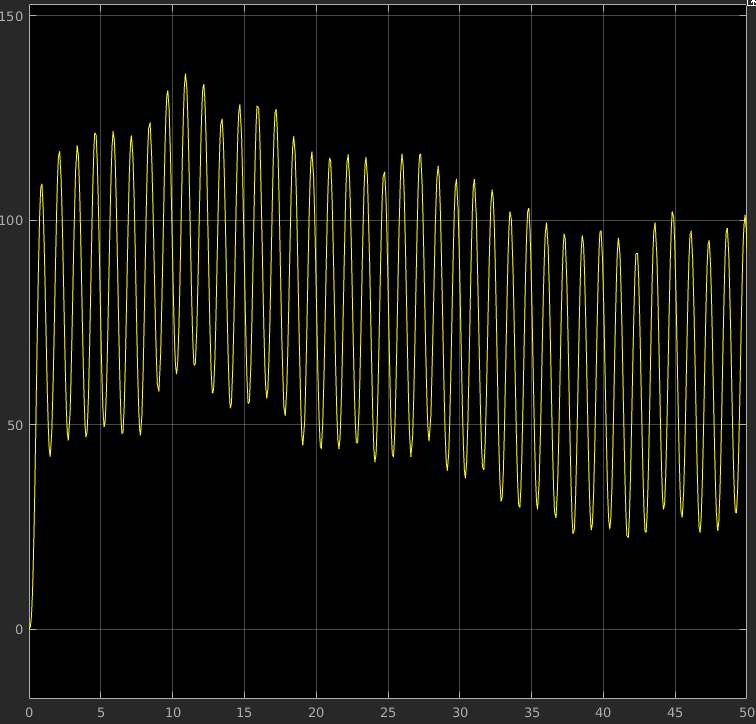
\includegraphics[width=0.7\textwidth]{pospendulum.png}
	\caption{Gráfica de posición del sistema mostrado en la figura 1. Se aprecia inestable a través del tiempo.}
\end{figure}

Es por esto que, para evitar las variaciones en el tiempo, se desarrollará un controlador para el sistema coo parte de esta práctica. Para poder realizar este controlador necesitamos definir variables de error, las cuales tienen como fin lograr encontrar la diferencia entre la posición verdadera del sistema en cuestión y la posición ideal que será expresada como una función del tiempo. La posición de nuestro sistema puede ser modelada, idealmente, por la función trigonométrica seno. Estas dos funciones de posición se compararán para lograr así modificar la señal de salida.

Al igual que la posición, nuestra velocidad también se comparará con la velocidad ideal modelada como la primer derivada de nuestra posición, partiendo de dinámica básica. La ecuación que describirá nuestra aproximación lineal del sistema, aunado a los errores será la siguiente:

\begin{align}
	u = \frac{1}{k_3} (k_1 sin(e_1 + y_r(t)) + k_2 e_2 + y_r''(t) - a_1 e_1 - a_2 e_2)
\end{align}

Esta ecuación se obtiene a partir del sistema del péndulo con el que iniciamos, sin embargo las variables $e_1$ y $e_2$ se definen como variables de error, las cuales son las diferencias de las que hablábamos anteriormente. Podemos apreciar que los errores definidos tienen cierto "peso", el cual nos dice qué tanto afecta cada uno a la salida final del sistema. Estas sumas ponderadas las tomaremos en cuenta más adelante en la sección de \textit{Errores y sus sumas ponderadas}. La salida final, $u(t)$, es la retroalimentación que se llevará al sistema original para que así modifique su comportamiento de acuerdo a la ecuación (1).

\section*{Desarrollo}

Para la implementación de este sistema de control se utiliza el mismo sistema del péndulo con el que ya contamos como muestra la figura 1, sin embargo, en lugar de tener una señal de entrada como se muestra, esta será reemplazada por la salida de nuestro controlador, aquello que hemos definido como $u(t)$.

\begin{figure}[H]
	\centering
	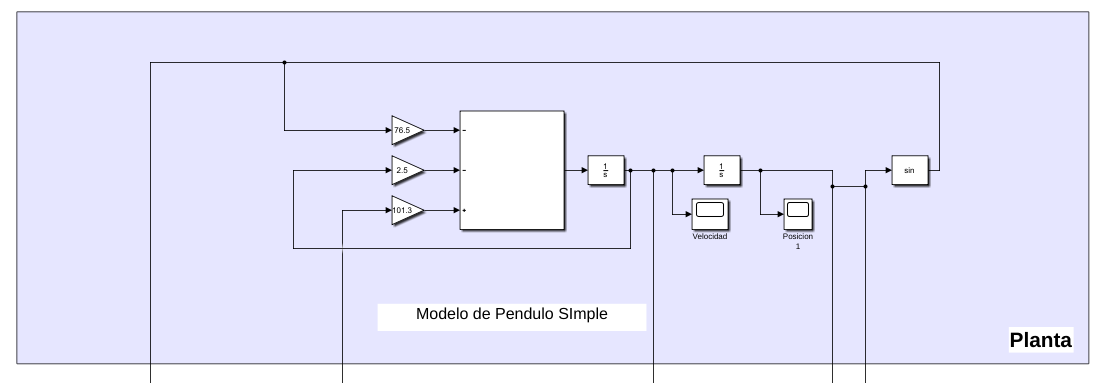
\includegraphics[width=0.9\textwidth]{plant.png}
	\caption{Señal de entrada del sistema original modificada.}
\end{figure}

Es notorio que algunas señales se han enviado a otros lugares, esto es debido a la necesidad que tiene nuestro controlador de conocer los estados de estas variables para así poder determinar otras variables, como los errores definidos. A continuación se muestra el sistema diseñado para controlar al péndulo.

\begin{figure}[H]
	\centering
	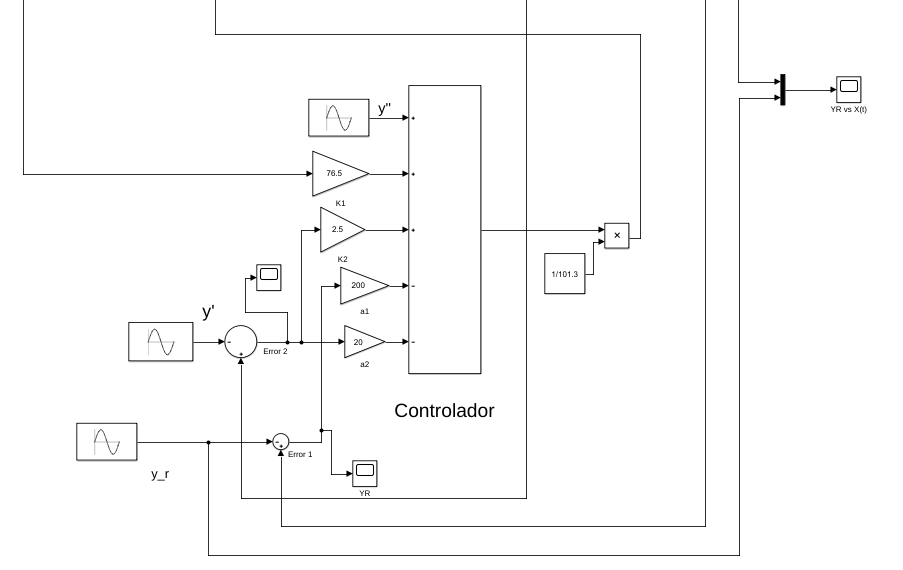
\includegraphics[width=\textwidth]{controller.png}
	\caption{Diseño del controlador.}
\end{figure}

\begin{figure}[H]
	\centering
	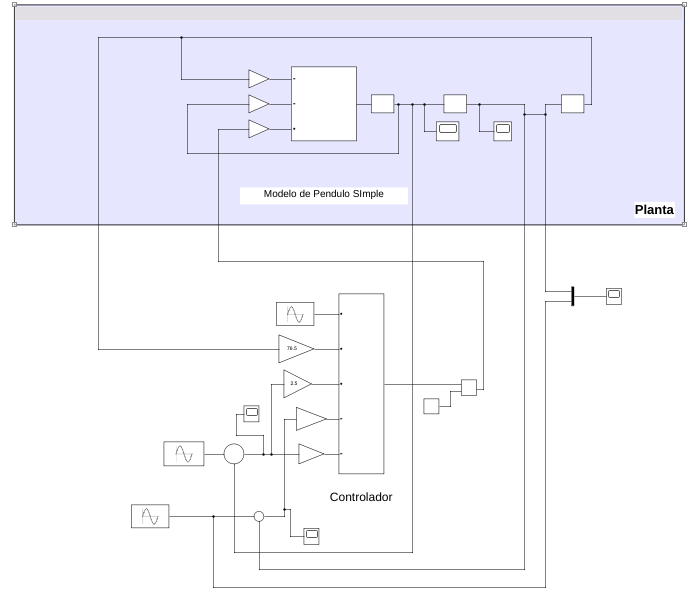
\includegraphics[width=\textwidth]{system.png}
	\caption{Imagen del sistema completo y las relaciones de señales que existen en él.}
\end{figure}
\subsection*{Análisis gráfico}
Ahora, ya implementado nuestro sistema de control, podemos realizar una comparación de las posiciones que teníamos antes (figura 2) y la que tenemos con el mismo sistema (figura 6):

\begin{figure}[H]
	\centering
	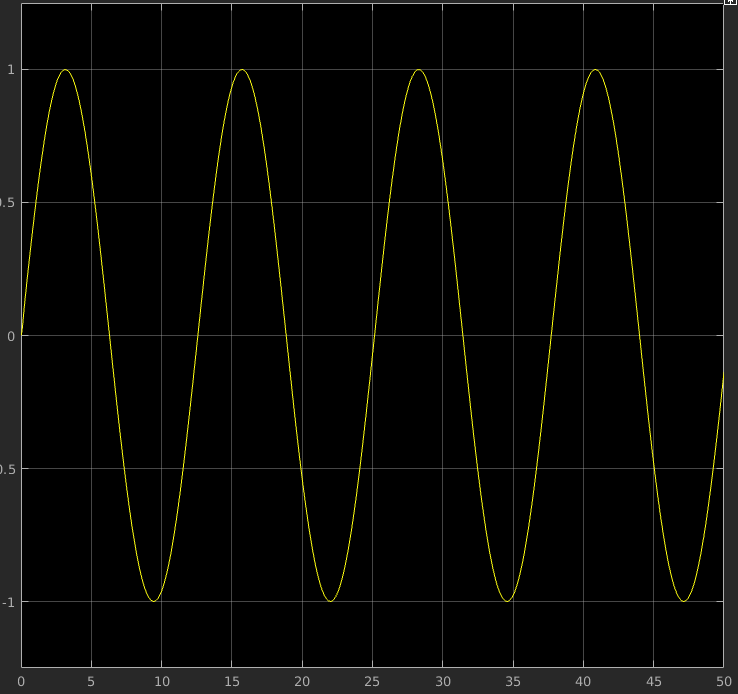
\includegraphics[width=0.4\textwidth]{posnew.png}
	\caption{Posición estable a través del tiempo.}
\end{figure}

Si se realiza la comparación entre nuestra función de referencia, $y_r(t)$, y la posición de nuestro sistemas podemos notar que la diferencia es muy pequeña.

\begin{figure}[H]
	\centering
	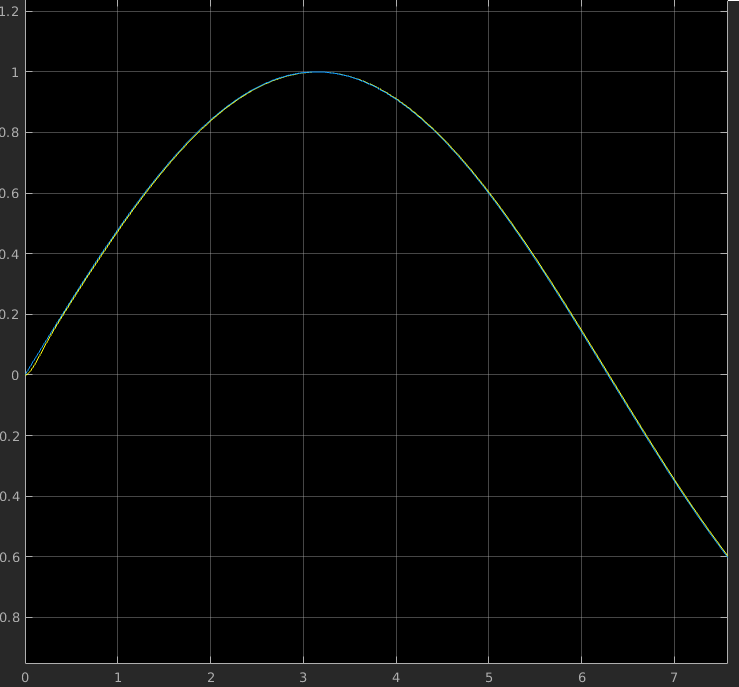
\includegraphics[width=0.5\textwidth]{yrvsx.png}
	\caption{En amarillo se muestra la posición del sistema y en azul la función de referencia.}
\end{figure}

\subsection*{Errores y sus sumas ponderadas}
Si deseamos conocer el error que presentan estas gráficas entre sí podemos observarlo gracias a los errores que hemos definido en el modelado de nuestro sistema de control. Si recordamos las constanes que multiplican a nuestros erroes, podemos entender que estas sumas ponderadas afectarán en distina manera al sistema dependiendo del valor de éstas constantes. A continuación veremos dos casos en donde podemos apreciar ambos errores graficados con distintos valores de $a_1$ y $a_2$.

\begin{figure}[H]
	\centering
	\begin{subfigure}[b]{0.49\linewidth}
		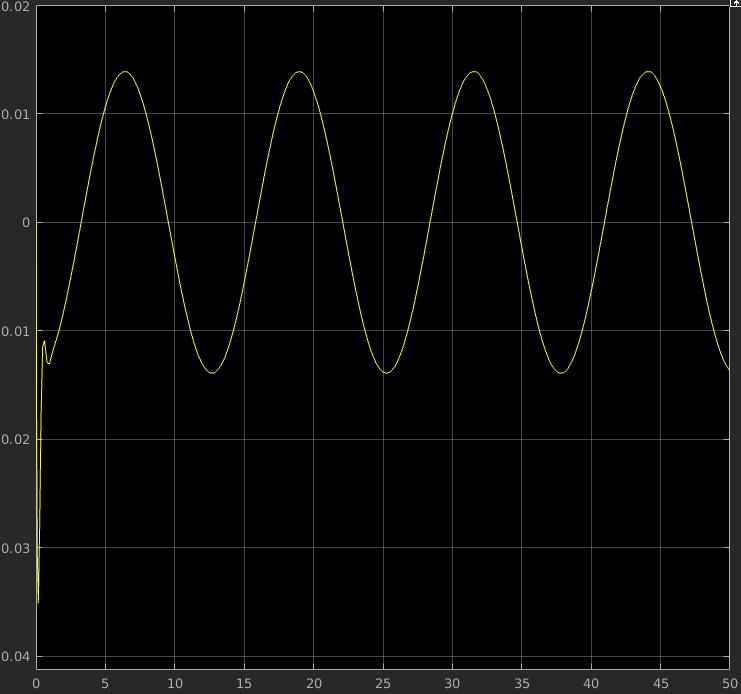
\includegraphics[width=\linewidth]{e1a90.png}
		\caption{Error 1}
	\end{subfigure}
	\begin{subfigure}[b]{0.49\linewidth}
		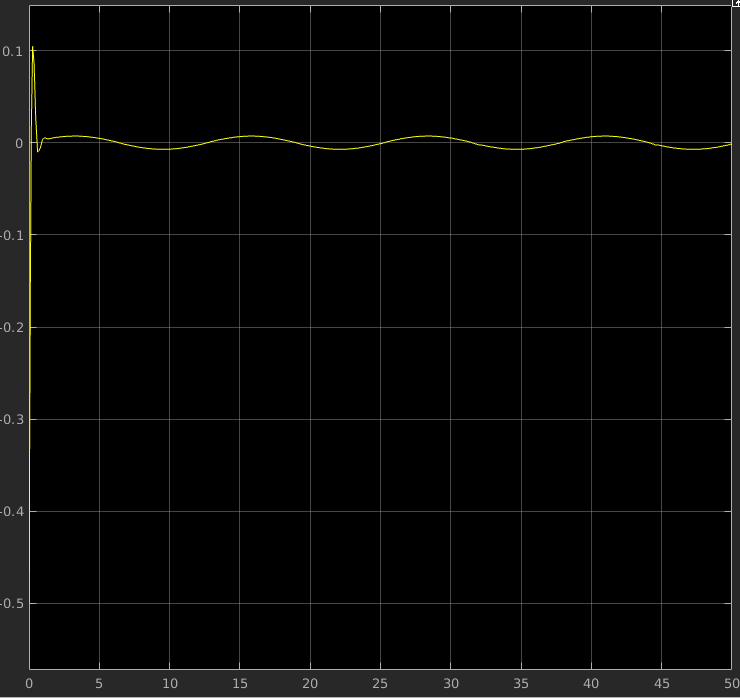
\includegraphics[width=\linewidth]{e2a90.png}
		\caption{Error 2}
	\end{subfigure}
	\caption{Gráficas de ambos errores cuando $a_1 = 90$ y $a_2 = 10$}
\end{figure}


\begin{figure}[H]
	\centering
	\begin{subfigure}[b]{0.49\linewidth}
		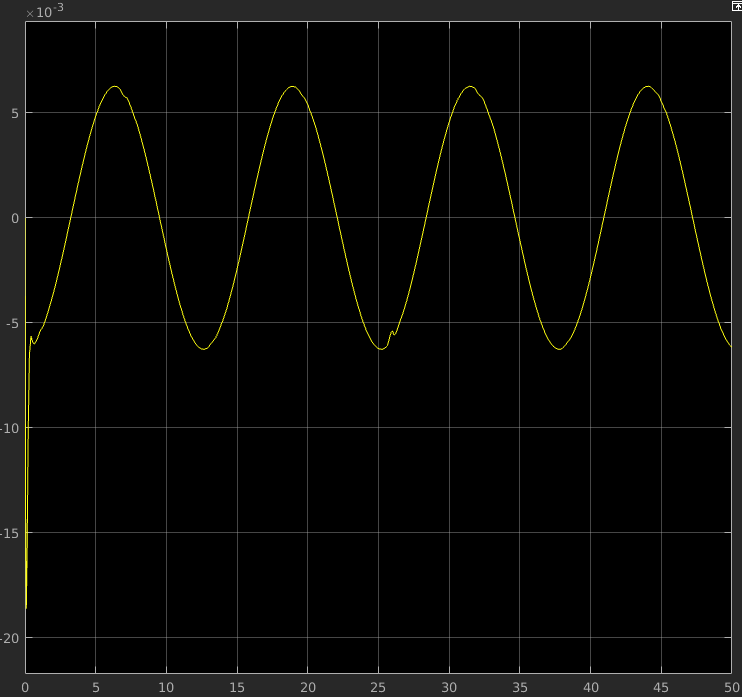
\includegraphics[width=\linewidth]{e1a200.png}
		\caption{Error 1}
	\end{subfigure}
	\begin{subfigure}[b]{0.49\linewidth}
		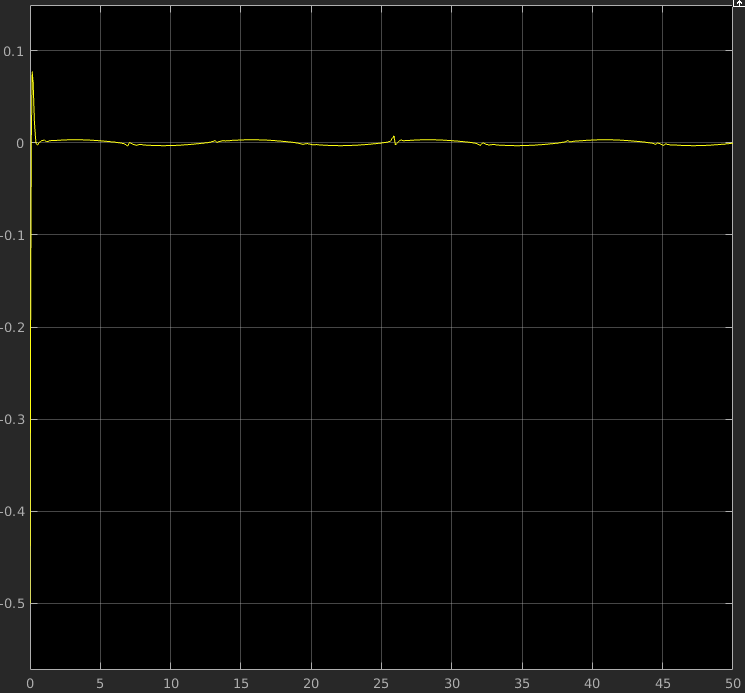
\includegraphics[width=\linewidth]{e2a200.png}
		\caption{Error 2}
	\end{subfigure}
	\caption{Gráficas de ambos errores cuando $a_1 = 200$ y $a_2 = 20$}
\end{figure}

Como podemos observar, el "peso" que se le da a cada error cuando éste es retroalimentado al sistema es de gran importancia, si ponemos atención a la escala que se marca cuando $a_1 = 200$ y $a_2 = 20$, podemos observar que ambos errores son considerablemente pequeños, a diferencia de los errores que se muestran cuando las constantes son más pequeñas. Es claro que no podemos simplemente aumentar estas constantes sin limitaciones, es por eso que debemos de tener bien claro cómmo funciona nuestro sistema y así modelar algo que sea más sencillo de modificar.

\section*{Conclusión}
Los sistemas de control son sistemas dinámicos que se basan en la retroalimentación, a veces pueden ser complejos, sin embargo es necesario entenderlos a fondo para evitar diseñar algo que no logre cumplir su función. Como fue posible observar a partir de la figura 8 y 9, estos sistemas son capaces de reducir y cambiar la salida de otro sistema que intenta comportarse de una manera pero no le es posible por perturbaciones externas. Así es como se tiene que lidiar con las adversidades naturales a las que estamos sujetos en el mundo real y, a pesar de que no son totalmente perfectas, son lo suficientemente buenas para hacernos viajar a través de continentes y poner satélites en órbita.
%%%%%  Bib
\renewcommand\refname{Referencias}
\printbibliography
\end{document}
